\documentclass[12pt]{article}

\usepackage{answers}
\usepackage{setspace}
\usepackage{graphicx}
\usepackage{enumitem}
\usepackage{multicol}
\usepackage{textcomp}
\usepackage{mathrsfs}
\usepackage{adjustbox}
\usepackage{svg}
\usepackage[margin=1in]{geometry}
\usepackage{amsmath,amsthm,amssymb}

\newcommand{\N}{\mathbb{N}}
\newcommand{\Z}{\mathbb{Z}}
\newcommand{\C}{\mathbb{C}}
\newcommand{\R}{\mathbb{R}}
\newcommand{\Q}{\mathbb{Q}}

\DeclareMathOperator{\sech}{sech}
\DeclareMathOperator{\csch}{csch}

\newenvironment{theorem}[2][Theorem]{\begin{trivlist}
\item[\hskip \labelsep {\bfseries #1}\hskip \labelsep {\bfseries #2.}]}{\end{trivlist}}
\newenvironment{definition}[2][Definition]{\begin{trivlist}
\item[\hskip \labelsep {\bfseries #1}\hskip \labelsep {\bfseries #2.}]}{\end{trivlist}}
\newenvironment{proposition}[2][Proposition]{\begin{trivlist}
\item[\hskip \labelsep {\bfseries #1}\hskip \labelsep {\bfseries #2.}]}{\end{trivlist}}
\newenvironment{lemma}[2][Lemma]{\begin{trivlist}
\item[\hskip \labelsep {\bfseries #1}\hskip \labelsep {\bfseries #2.}]}{\end{trivlist}}
\newenvironment{exercise}[2][Exercise]{\begin{trivlist}
\item[\hskip \labelsep {\bfseries #1}\hskip \labelsep {\bfseries #2.}]}{\end{trivlist}}
\newenvironment{solution}[2][Solution]{ \begin{trivlist}
\item[\hskip \labelsep {\bfseries #1}]}{\end{trivlist}}
\newenvironment{problem}[2][Problem]{\begin{trivlist}
\item[\hskip \labelsep {\bfseries #1}\hskip \labelsep {\bfseries #2.}]}{\end{trivlist}}
\newenvironment{question}[2][Question]{\begin{trivlist}
\item[\hskip \labelsep {\bfseries #1}\hskip \labelsep {\bfseries #2.}]}{\end{trivlist}}
\newenvironment{corollary}[2][Corollary]{\begin{trivlist}
\item[\hskip \labelsep {\bfseries #1}\hskip \labelsep {\bfseries #2.}]}{\end{trivlist}}

\begin{document}

% --------------------------------------------------------------
%                         Start here
% --------------------------------------------------------------

\title{Assignment 1}%replace with the appropriate homework number
\author{Aditya Arora\\ %replace with your name
Winter 2018} %if necessary, replace with your course title

\maketitle
\begin{center}
    $Absque\ sudore\ et\ labore\ nullum\ opus\ perfectum\ est$
\end{center}
%Below is an example of the problem environment
\begin{problem}{1}
Prove or Disprove:
\begin{enumerate}[label=\alph*)]
    \item $ R \subseteq \ S\ \Leftrightarrow \ R \ \subseteq ((S-T)\cup(R\ \cap\ T)) $
    \item $(A \cap B) \subseteq (B \cap C) \longrightarrow (A \subseteq C)$
    \item $A \in B \wedge B \in C \longrightarrow A \in C$
    \item $A \in B \wedge B \in C \longrightarrow A \subseteq C$
    \item $A \in B \wedge B \subseteq C \longrightarrow A \in C$
    \item $A \in B \wedge B \subseteq C \longrightarrow A \subseteq C$
\end{enumerate}
\end{problem}

%Below is the solution environment
\begin{solution}{1}
\item[]
\begin{enumerate}[label=\alph*)]
\item This can be disproved by a counter example $$R = \{1,2,3,4\},\ S = \{1,2,3\},\ T = \{4\} \\$$
The right hand side is:
$R \subseteq \{1,2,3\} \cup \{4\}$ which is $R \subseteq \{1,2,3,4\} \\$ which is true, but on the other hand the left hand side $R \subseteq S$ is false and $R \nsubseteq S$ \\
Thus, the given statement is false

\item This can be disproved by a counter example $$A = \{1,2,3,4\},\ C = \{1,2,3\},\ B = \{1,2,3\} \\$$
The left hand side is:
$\{1,2,3\} \subseteq \{1,2,3\}$ which is true, but on the other hand the right hand side $A \subseteq B$ is false and $A \nsubseteq B$ \\
Thus, the given statement is false

\item This can be disproved by a counter example $$A = \{1,2,3,4\},\ B = \{\{1,2,3,4\},\{0\}\},\ C = \{\{\{1,2,3,4\},\{0\}\}\} \\$$
The left hand side is:
$A \in B \wedge B \in C$ which is true, but on the other hand the right hand side $A \in C$ is false and $A \notin C$ \\
Thus, the given statement is false

\item This can be disproved by a counter example $$A = \{1,2,3,4\},\ B = \{\{1,2,3,4\},\{0\}\},\ C = \{\{\{1,2,3,4\},\{0\}\}\} \\$$
The left hand side is:
$A \in B \wedge B \in C$ which is true, but on the other hand the right hand side $A \subseteq C$ is false and $A \nsubseteq C$ \\
Thus, the given statement is false

\item if $A \in B$ and $B \subseteq C$ then we can say that $\forall_x\ in\ B$, $x$ also exists in $C$ and since $A$ is an element of $B$ we can safely say that $A$ is an element of $C$ and hence $A \in C$

\item This can be disproved by a counter example $$A = 1,\ B = \{1,2,3,4\},\ C = \{1,2,3,4\}$$
The left hand side is:
$A \in B \wedge B \subseteq C$ which is true, but on the other hand the right hand side $A \subseteq C$ is false and $A \nsubseteq C$ \\
Thus, the given statement is false
\end{enumerate}
\end{solution}

\vskip 0.5in

\begin{problem}{2}
Given sets $A$ and $B$, under what conditions does $A\ -\ B\ = B\ -\ A$?. Prove that this is the only conditions under which this is true
\end{problem}
\begin{solution}{2}
\item[]
If $A - B$ = $B - A$ then \\ for any $x\in\ A - B$ = $B - A$ we know, $x \in A$ and $x \in B$ and $x\notin A$ and $x\notin B$.\\ That's a contradiction so $A - B$ = $B - A$ is empty.
\\
Thus there are no elements in $A$ that are not in $B$. In other words $A$ is a subset of $B$. \\ Likewise there are no elements of $B$ that are in $A$. So $B$ is a subset of $A$.
\\
\indent So $A=B$
\end{solution}

\pagebreak


\begin{problem}{3}
\item[]
\begin{enumerate}[label=\alph*)]
    \item Given $ f \colon \ A \longrightarrow B$, what is the relation between $f$'s co-domain and it's image if $f$ is
    \begin{enumerate}[label=(\roman*)]
    \item injective
    \item surjective
    \item bijective
    \end{enumerate}
    \item Given $ f \colon \ A \longrightarrow B$, what is the relation between the image of $f^{-1}$ and the domain of $f$ if $f$ is
    \begin{enumerate}[label=(\roman*)]
    \item injective
    \item surjective
    \item bijective
    \end{enumerate}
\end{enumerate}
\end{problem}
\begin{solution}{3}
\item[]
\begin{enumerate}[label=\alph*)]
\item
    \begin{enumerate}[label=(\roman*)]
        \item injective : The image is a subset of the co-domain
        \item surjective: The image is equal to the co-domain
        \item bijective: The image is equal to the co-domain
        \end{enumerate}
\item
    \begin{enumerate}[label=(\roman*)]
        \item injective : The image is equal to the domain
        \item surjective: The inverse of $f$ is not defined
        \item bijective: The image is equal to the domain
        \end{enumerate}
\end{enumerate}
\end{solution}
\vskip 0.5in
\begin{problem}{4} Given sets $X,\ Y$ such that $X \subseteq Y$. Prove or disprove:
% \item[]
\begin{enumerate}[label=\alph*)]
    \item There exists an injection $ f \colon \ X \longrightarrow Y$
    \item There exists an surjection $ f \colon \ Y \longrightarrow X$
\end{enumerate}
\end{problem}
\begin{solution}{4}
\item[]
We are given that $X \subseteq Y$ thus, we can say cardinality($X$) $\leq$ cardinality($Y$)
\begin{enumerate}[label=\alph*)]
    \item From above we can clearly say $\forall x \in X\ \exists\ y \in Y$ such that such that each $x$ is mapped to a unique $y$ and there might be elements in Y that have no pre-image in X.\\
    Thus an injective function exists
    \item The given statement can be disproved by taking a counter example. \\ If the subset $X$ is empty then there does not exist a well defined surjection from $Y$ to $X$.
    Therefore the given statement is not true
\end{enumerate}
\end{solution}

\vskip 0.5in

\begin{problem}{5}Given the following functions, are they: injective, surjective, bijective, or none of these?
\item[]
\begin{enumerate}[label=\alph*)]
    \item $ f \colon \ \N \longrightarrow \N$ where
    $ f \colon \ x \mapsto x$
    \item $ g \colon \ \N \longrightarrow \N$ where
    $ g \colon \ x \mapsto x^2$
    \item $h \colon \ \Q^+ \longrightarrow \Q^+$ where
    $ f \colon \ x \mapsto 1/x$
    \item If it is possible to compose $f$ and $g$, $f$ and $h$ and $g$ and $h$ what is the result of the composition. If not explain why not?
\end{enumerate}
\end{problem}
\begin{solution}{5}
\item[]
\begin{enumerate}[label=\alph*)]
    \item
    INJECTIVE:
        If $f(x_1) = f(x_2)$ then it implies that $x_1 = x_2$\\
    SURJECTIVE:
        Range of $f(x)$ is clearly $\N$ which is same as it's co-domain.\\
    Since $f(x)$ is both injective and surjective, we can say that it is bijective
    \item
    INJECTIVE:
        If $g(x_1) = g(x_2)$ then it implies that $x_1 = x_2$ since we are only restricted to the positive square root in the set of natural numbers \\
    SURJECTIVE: We cannot say it is surjective since the numbers in $\N$ which are not perfect squares do not lie in the range of $g(x)$ \\
    Thus $g(x)$ is only injective
    \item
    INJECTIVE:
        If $h(x_1) = h(x_2)$ then it implies that $1/x_1 = 1/x_2 \implies x_1 = x_2$\\
    SURJECTIVE:
        Range of $h(x)$ is clearly $\Q^+$ since all numbers in $\Q^+$ also have their inverses in $\Q^+$. This implies that $h(x)$ is surjective\\
    Since $f(x)$ is both injective and surjective, we can say that it is bijective
    \item
    \begin{enumerate}[label=(\roman*)]
        \item $f \circ g \colon \N \longrightarrow \N$ where $ f \circ g \colon \ x \longrightarrow x^2$
        \item $f \circ h \colon \N \longrightarrow \Q^+$ where $ f \circ h \colon \ x \longrightarrow 1/x$
        \item $g \circ h \colon \N \longrightarrow \Q^+$ where $ g \circ h \colon \ x \longrightarrow 1/x^2$
    \end{enumerate}
\end{enumerate}
\end{solution}


\vskip 0.5in

\begin{problem}{6}Prove or disprove: Given a strict partial order ($X,<$), the pair ($X,<^{ref}$) is a partial order

\end{problem}
\begin{solution}{6}
Since ($X,<$) is a strict partial order, thus we can say that we will need to add minimum number of terms for the reflexive closure.\\ The terms that we will add will be of the form $(x,x)\ \forall x \in X$.
Adding these reflexive terms will make ($X,<^{ref}$) reflexive. \\
But adding these terms won't affect transitivity since $xRx \wedge xRy \Rightarrow xRy$ but $xRy$ is already in the relation so the relation. Thus, ($X,<^{ref}$) also remains transitive
\\
Also all the new added reflexive terms will inherently exhibit anti-symmetry.
\\
Therefore ($X,<^{ref}$) is reflexive, anti-symmetric, transitive.
\\
Thus according to the definition of a partial order,  ($X,<^{ref}$) is a partial order
\end{solution}

\pagebreak

\begin{problem}{7}
Consider the set of letter grades G = \{ A, B, C, D, F, INC, WD, AEG \}. A, B, C, D, and F are what you would intuitively think they are, with A “better than” B, which is “better than” C, etc. \\ \vskip 0.05in
INC means “Incomplete”. This means the final grade has not yet been assigned because some outstanding work is missing. After the outstanding work is done, a final grade will be assigned. If the outstanding work is never done, then an INC changes to an F after two terms. Is an INC “better than” an F? Well, it is at least “better than or equal to” an F, since it will never get worse than F, and let’s be honest: it’s really “better than” F because (a) it is easier to explain away an INC during an interview than an F (“I was sick an so did not complete ...; my average prior to that was -state something plausible and consistent with other grades. ....”) (b) the student will probably do better than an F when the outstanding work is submitted (otherwise why bother do the work, since it will automatically change to an F in two terms); in the meantime, reason (a) says an F now is “worse than” an F later. Is INC “better than” a D? That is harder to argue. It could become an F. It means there is outstanding work and it will become an F if that work is not completed. We will therefore claim that INC is “better than or equal to” a D but cannot say more than that with respect to D. How about a B or C? Realistically, we cannot claim any relationship between INC and B or C, since we do not know what the result of completing the outstanding work will be, so there can be no “better than” relation between those grades and INC. Finally, there is A? Is A “better than” INC? Clearly it is, because there is no grade better than A. Even when the outstanding work is done, the best the INC can become is an A, and an A now means there is nothing to even explain in an interview. Ergo, A is “better than” INC. \vskip 0.2in
WD means “Withdrawn” and so the class was attended long enough that it will not be removed from a transcript, but not so long that a final-grade assessment will be made. It is somewhat awkward to have on a transcript (better to have dropped prior to the drop deadline), but far better than a failing grade on the transcript. Therefore WD is “better than” F. Is it better than D? Almost certainly it is. D is not a great grade. It is a pass, but barely. In a traditional setting, it means: pass, but this course cannot be used as a prerequisite for some subsequent course. If it is for an elective, unrelated to a major, it may be OK, but WD is arguably better since it says that the student recognized that it was better to drop the course than not. Ergo, WD is “better than” D. As with INC, it is not really comparable to C, since C is an OK, but not good, grade. How about B? B is a good grade. Is it better to have withdrawn from a course of got a B? This is unclear. It is probably reasonable to claim that B is “better than or equal to” a WD. \vskip 0.2in
Finally, AEG is a curious grade that hopefully you will never experience, but is useful in some circumstances. AEG is short for “Aegrotat” which is Latin for “s/he is ill.” It is a grade that is awarded when a student has demonstrated enough ability to show that s/he has passed the course, but no better granularity is possible on the grade because there is insufficient information to make that determination. It is almost like a “pass” in a “pass/fail” system, except that what is it really saying is “the grade is somewhere between A and D but we do not have enough information to say where (because the student was ill).” Given that it is often viewed as a “pass” in a “pass/fail” system, it is reasonable to argure that an AEG is “at least as good as” a C, but not much more can be stated about it.
Given the information above:
\item[]
\begin{enumerate}[label=\alph*)]
    \item Draw a graph of the “better than” relation for the set G.
    \item Draw a graph of the “better than or equal to” relation for the set G.
    \item Over the set G, for each of the relations (“better than” and “better than or equal to”), is there a least upper bound and a greatest lower bound, and if so what are they?
    \item Over the set G \textminus  \{A, F\}, for each of the relations, what are the minimal and maximal elements?
    \item Are the relations partial orders? Is there any missing information and/or information you are assuming that might affect that answer?
\end{enumerate}
\end{problem}
\begin{solution}{7}
\item[]
\begin{enumerate}[label=\alph*)]
\item \begin{minipage}[t]{\linewidth}
          \raggedright
          \adjustbox{valign=t}{%
            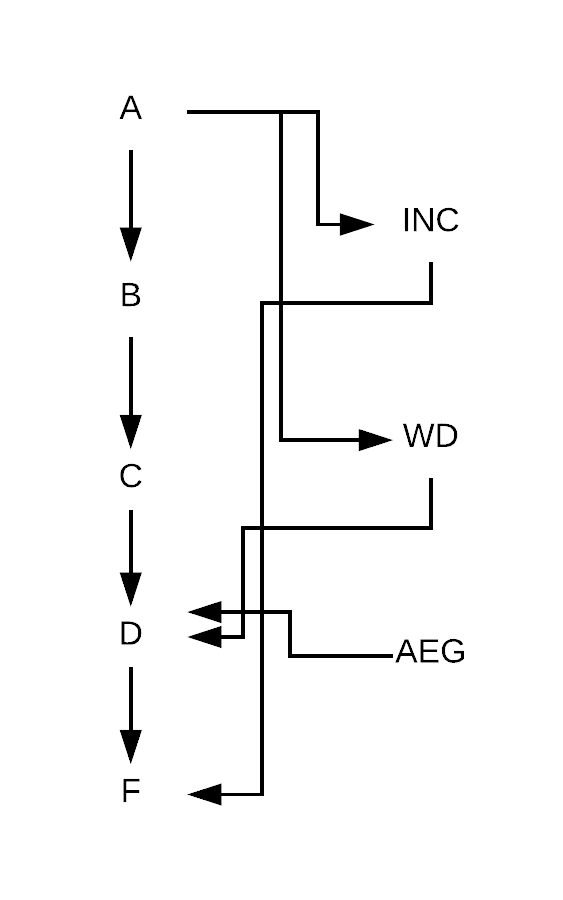
\includegraphics[scale=0.3]{(a)}%\\
          }
          Better Than Relation over G\\
           \footnotesize Note: Transitive relations excluded to preserve clarity
          \end{minipage}
\item
\begin{minipage}[t]{\linewidth}
          \raggedright
          \adjustbox{valign=t}{%
            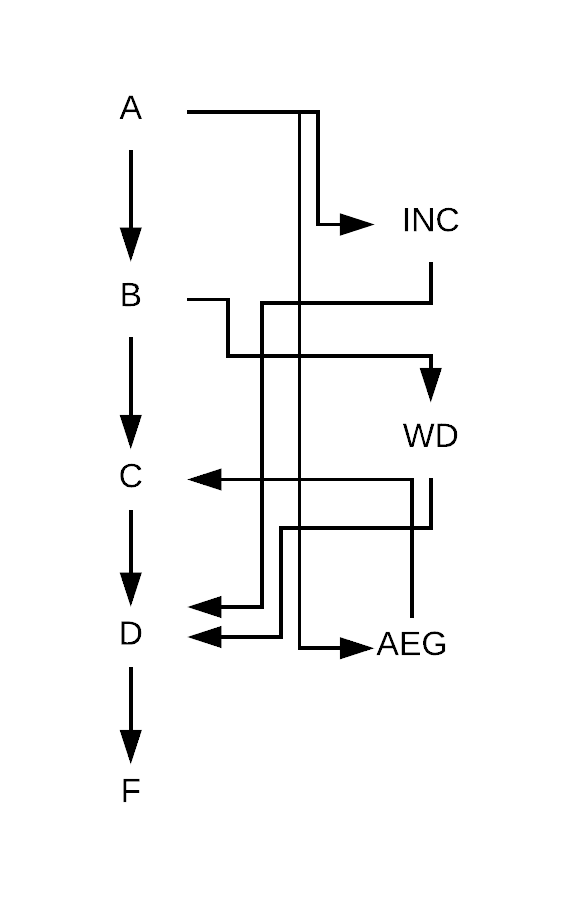
\includegraphics[scale=0.3]{(b)}%\\
          }
          Better Than or Equal to Relation over G\\
           \footnotesize Note: Transitive relations and self relations excluded to preserve clarity
          \end{minipage}

\item The LUB in the better than relationship is $A$. As for the GLB in the better than relation's GLB is $F$. In the better than or equal to relationship, LUB is $A$ and GLB does not exist since we cannot compare $AEG$ and $F$

\item \begin{enumerate}[label=\roman*)]
\item For the "better than" relation: \\Minimal elements: \{B, INC, AEG, WD\};\\
Maximal elements: \{D\}
\item For the "better than or equal to" relation: \\Minimal elements: \{B, INC, AEG\};\\
Maximal elements: \{D\}
\end{enumerate}
\item "Better Than" relation is a partial order but due to lack of information the "Better Than or Equal To" is not a partial order
\end{enumerate}
\end{solution}
\pagebreak


\begin{problem}{8}Given $R, S \subseteq A^2$ are relations on $A$. Define $T \subseteq A^2$ such that \\ $xTy \Leftrightarrow (xRy \wedge xSy)$. \\Prove or disprove: If  $R$ and $S$ are equivalence relations,then $T$ is also an equivalence relation.
\end{problem}
\begin{solution}{8}
Suppose $R$ and $S$ are both equivalence relations on a set A. We will show that $R$ and $S$ both being equivalence relations on the set A implies that $T$ is also an equivalence relation.
\vskip 0.2in
It is immediately apparent that since $R$ and $S$ are equivalence relations then:

$x \in A \Rightarrow (xRx)\wedge(xSx)\Rightarrow ((x,x) \in R) \wedge ((x,x) \in S) \Rightarrow (x,x) \in T$
\vskip 0.1in
Thus $x \in A \Rightarrow (x,x) \in T$, therefore $T$ is reflexive.
\vskip 0.2in
Now suppose $(x,y) \in T \Rightarrow (xRy)\wedge(xSy)\Rightarrow(yRx)\wedge(ySx)$ \vskip 0.1in
[Since both $R$ and $S$ are symmetric]
$\Rightarrow((y,x) \in R) \wedge ((y,x) \in S) \Rightarrow (y,x) \in T$
\vskip 0.2in
Since both $R$ and $S$ are symmetric, $T$ will also be symmetric as shown above
\vskip 0.2in
Finally suppose $((x,y) \in T \wedge (y,z) \in T) \Rightarrow ((xRy)\wedge(xSy))\wedge((yRz)\wedge(ySz))\Rightarrow(xRz)\wedge(xSz)$ \vskip 0.1in
[Since both $R$ and $S$ are transitive]
$\Rightarrow((x,z) \in R) \wedge ((x,z) \in S) \Rightarrow (x,z) \in T$
Thus we have shown $T$ is transitive

It follows that $T$ is an equivalence relation since it is reflexive, symmetric and transitive.  $\square$
\end{solution}

\vskip 0.1in
\pagebreak

\begin{problem}{9}
 Given poset $(X, \le)$, prove or disprove:
\item[]
\begin{enumerate}[label=\alph*)]
    \item $x \ge y \Leftrightarrow y \le^{\text{--}1} x$
    \item $x \ge y \Leftrightarrow y \le' x$
    \item $x < y \Leftrightarrow y \le' x$
    \item $x > y \Leftrightarrow y (\le^{\text{--}1})' x$
    \item $x > y \Leftrightarrow y (\le')^{\text{--}1} x$
\end{enumerate}
\end{problem}
\begin{solution}{9}
Assuming this stands True for all posets:
\begin{enumerate}[label=\alph*)]
    \item $x \ge y \Leftrightarrow x (\le)^{-1} y$ , therefore it cannot imply $y \le^{\text{--}1} x$ \\
    $7 \ge 5 \Leftrightarrow 7 (\le)^{-1} 5$ , but $5 \nleqslant^{\text{--}1} 7$
    \item $x \ge y \Leftrightarrow x (<)' y$ , therefore it cannot imply $y \le' x$ \\
    $7 \ge 5 \Leftrightarrow 7 (<)' 5$ , but $5 \nless' 7$
    \item $x < y \Leftrightarrow y > x \Rightarrow (y \geq x \wedge y \neq x)$ , therefore by anti-symmetry it implies that $y \le^{\text{--}1} x$
    \item $x > y \Leftrightarrow x \leq^{-1} y \Leftrightarrow y (\le^{-1})' x$, this statement is inherently true as shown from earlier
    \item $x > y \Leftrightarrow x \le' y \Leftrightarrow y (\le')^{-1} x$, this statement is inherently true as shown from earlier
\end{enumerate}
\end{solution}
\vskip 0.1in
\begin{problem}{10}Given $X \subseteq \N, \forall_{x,y\in\N}\ x \le y \Leftrightarrow \exists_{z \in X} x+z=y$. Prove that,if $(X,\le)$ is a partial order:
\item[]
\begin{enumerate}[label=\alph*)]
    \item $0 \in X$
    \item $\forall_{x,y} (x \in X \wedge y \in X) \rightarrow x + y \in X$
\end{enumerate}
\end{problem}
\begin{solution}{7}
\item[]
\begin{enumerate}[label=\alph*)]
    \item Given $(X,\le)$ is a partial order we can say that $(X,\le)$ is reflexive over $X$,
    thus $$(x \le x \Leftrightarrow \exists_{z \in X} x+z=x) \Rightarrow (z = 0 \wedge z \in X) \Rightarrow 0 \in X$$
    \item Since $x,y \in X \wedge x \subseteq \N \Rightarrow x,y \in \N \Rightarrow x+y \in \N$\\
    Also $\exists_{z \in X}\ such\  that\ x + z = y$\\
    Thus going from right to left in the given bi-directional implication and using that $z=0$ \\
    $(x+y) + 0 = (x+y) \Leftrightarrow (x+y) \le (x+y)$\\ And since $(X, \le)$ is a partial order, $\le$ is reflexive,\\
    Therefore $\forall_{aRa}, a \in X$\\
    Therefore, $(x+y) \le (x+y) \Rightarrow (x+y) \in X$
\end{enumerate}
\end{solution}

\vskip 0.5in

\begin{problem}{11}Given partially ordered set $(X,\le)$, and $Y \subseteq X$, define a minimum element in $Y$ as:
\vskip 0.1in
$x$ is a minimum element in $Y \Leftrightarrow x \in Y \wedge \forall_{y \in Y}\ x \le y$
\vskip 0.1in
Note the difference between this definition and that of a minimal element ($x \in Y$ is a minimal element in $Y$ if  $\nexists_{y \in Y}\ y < x$). Prove or disprove:
\item[]
\begin{enumerate}[label=\alph*)]
    \item If x is a minimum element in Y then x is unique.
    \item If x is a minimum element in Y then x is a minimal element in Y .
    \item If x is a minimal element in Y then x is a minimum element in Y .
    \item If every nonempty subset of X has a minimum element, then X is totally ordered.
\end{enumerate}
\end{problem}
\begin{solution}{11}
\item[]
\begin{enumerate}[label=\alph*)]
    \item Let us assume that x is not unique, which means there exists z such that $z \in Y \wedge  \forall_{y \in Y}\ z \le y$ and since $x$ is also a minimum element $x \in Y \wedge \forall_{y \in Y}\ x \le y$ which implies that [after combining those 2 statements]: $x \le z \wedge z \le x \Rightarrow x$ = $z$. Therefore the minimum element is unique
    \item Since $x$ is a minimum element in $Y$ we can say that $ x \in Y \wedge \forall_{y \in Y}\ x \le y$ this clearly implies that there does not exist an element in $Y$ that is smaller than x $\nexists_{y \in Y}\ y < x$.\\ Therefore, x is also the minimal element
    \item Since $x$ is a minimal element in $Y$ we can say that $\nexists_{y \in Y}\ y < x$  this clearly implies that there does not exist an element in $Y$ that is smaller than x $ \Rightarrow \forall_{y \in Y}\ x \le y$.\\ Therefore, x is also the minimum element
    \item Given the fact that every subset has a minimum element, we can say that $\forall_{x_1,x_2} \in X$ for subset $A = \{x_1, x_2\}$ either: $x_1 \leq x_2$ or $x_2 \leq x_1$ and since this holds $\forall_{x_1,x_2} \in X$ we can imply that $X$ is totally ordered
\end{enumerate}
\end{solution}


\vskip 0.5in
\pagebreak
\begin{problem}{12}Given finite set A with cardinality N :
\item[]
\begin{enumerate}[label=\alph*)]
    \item How many distinct functions, $f \colon A \rightarrow A$, exist that map A to A?
    \item How many of these functions are injective? surjective? bijective?
    \item How many distinct binary relations, $R \subseteq A \times A$, exist on set A?
    \item How many of these relations are both symmetric and anti-symmetric?
    \item How many of these relations are both symmetric, anti-symmetric, and reflexive?
    \item How many of these relations are equivalence relations?
\end{enumerate}
\end{problem}
\begin{solution}{12}
\item[]
\begin{enumerate}[label=\alph*)]
    \item By elementary combinatorics we can say that every element in $A$ has $N$ choices for it's output, therefore total number of function = $N^N$
    \item
    \begin{enumerate}[label=(\roman*)]
        \item Injective Only: The first input has N choices, the next one has N choices as well and so on. Thus the total number of functions are: $N^N$
        \item Surjective Only: Since the size of domain and co-domain is same, all Surjective functions will be bijective by default. Therefore as explained below the total number of functions are: $N!$
        \item Bijective: The first input has N choices, the next one has N-1 choice and so on. Thus the total number of functions are: $N!$
    \end{enumerate}
    \item cardinality($A \times A$) = $N^2$, each element in that set may or may not be in the relation $R$ therefore total number of relations is $2^{N^2}$
    \item Since the relation is both symmetric and anti-symmetric this means $\forall_{x,y \in A}(xRy \Leftrightarrow yRx \wedge x = y)$ therefore the relation is $xRy \Leftrightarrow x = y$. Therefore the number of relations is $2^N$ since we can either choose or not choose any of the ($xRx\ \forall\ x \in A$)
    \item Extending from the previous part, there is only one relation that is symmetric, antisymmetric as well as reflexive
    \item Extending from above there is only one relation that is reflexive, symmetric, anti-symmetric as well as transitive i.e. an Equivalence class
\end{enumerate}
\end{solution}

% \vskip 0.5in

% \begin{problem}{12}
% \item[]
% \begin{enumerate}[label=\alph*)]
% \end{enumerate}
% \end{problem}
% \begin{solution}{7}
% \item[]
% \begin{enumerate}[label=\alph*)]
% \end{enumerate}
% \end{solution}




\end{document}
